\documentclass[a4paper, 11pt, titlepage]{jsarticle}
\usepackage[dvipdfmx]{graphicx}

\title{File 書き出し速度の測定}

\author{235718G 新里 伊武輝 }
\date{\today}

\begin{document}
\maketitle

\clearpage

\section{実行結果}
FIle書き出し速度の実行結果は図\ref{fig:filewrite1}に示す。

\begin{figure}[htbp]
	\centering
	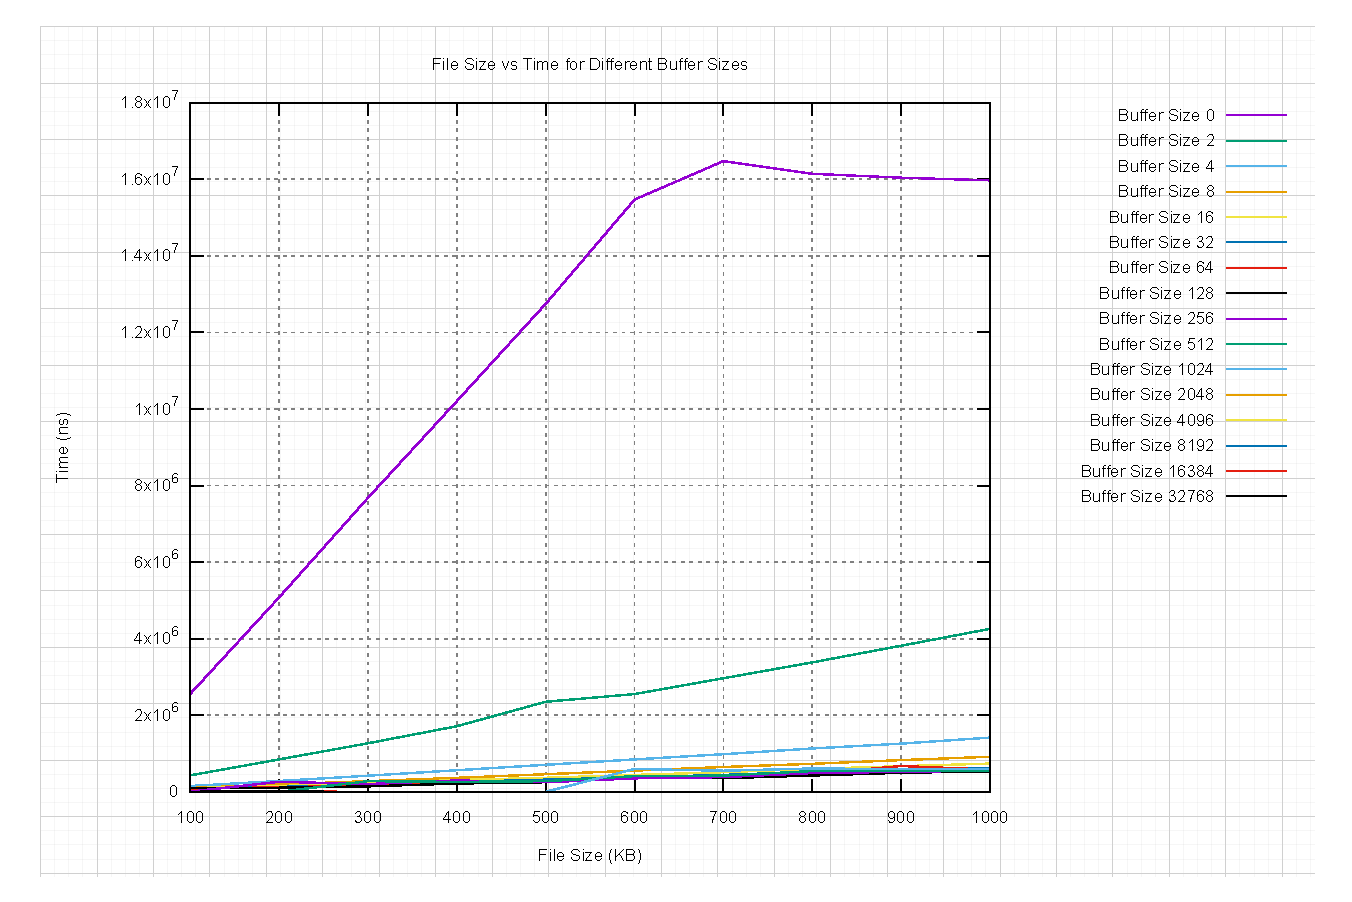
\includegraphics[width=120mm]{write_times.pdf}
	\caption{filewriteの実行時間}
	\label{fig:filewrite1}
\end{figure}

\section{考察}
Bufferedの影響を測定するのに適切なファイルの大きさは、File書き込みにおいては比較的にFile Sizeが大きい100KBから1000KBまでの範囲として、コンピュータのメモリ管理が2の累乗に基づいているので、bufferの大きさは0,2,4,...,32768byteの2の累乗とした。

図\ref{fig:filewrite1}より、UnBufferedとBufferedではBufferedの方がはるかにFile書き出し速度が速いことがわかる。また、どのBufferのサイズでFIle Sizeと書き出しの実行時間は比例関係であり、Bufferのサイズが大きければ大きいほどFile Sizeによる実行速度の遅延の影響を受けにくくなる。
Bufferのサイズが大きいほどFile Sizeの書き出しの効率は上がるが、Bufferの分割のサイズを適切なサイズにしないとオーベーヘッドの影響を大きく受けることになる。

\end{document}
